\documentclass[12pt]{report}
\usepackage{hyperref}
\hypersetup{
	colorlinks=true,
	linkcolor=blue,
	filecolor=magenta,      
	urlcolor=cyan,
	pdftitle={Overleaf Example},
	pdfpagemode=FullScreen,
}
\usepackage{csquotes}
\usepackage{graphicx}

\title{AI code generation report}
\author{Roblox prime numbers:\\\small{Oleh Basystyi}\\\small{Anna Stasyshyn}
\\\small{Artur Rudish}\\\small{Anton Valihurskyi}\\\small{Maksym Zhuk}}
\date{April 2024}
\begin{document}
	\maketitle	
	\renewcommand{\thesection}{\arabic{section}}
	\section{Introduction}
	\qquad In this little survey out team have researched AI's capability to solve CodeWars tasks of different difficulty (primarily 7, 6, 5, 4 kyu) and different CodeWars cagtegories:
	\begin{itemize}
		\itemsep0em 
		\item Algorithms
		\item Strings
		\item Arrays
		\item Mathematics
		\item Linear Algebra
		\item Dynamic Programming
		\item Data Structures
	\end{itemize}
	\qquad As AIs we used \textit{GPT-3.5, GPT-4, Claude} and \textit{Gemini} to create aggregated conslusion about AI code generation. Also we researched two ways of writting prompts to solve problems like this: templated and manual that must be used in different cases
	
	\pagebreak
	\section{Setup of experiments and general conclusions}
	\qquad To carefully carry out experiments we have set up \href{https://docs.google.com/spreadsheets/d/1qXPyAJsOOpmtxIoGqObwG5mTaLU3IWO0SQRGbjZPhEc/edit#gid=0}{google sheets table} to log data about AI performance on solving particular tasks by following metrics: \textit{Used prompts to solve problem, Number of times whan AI returned code that hadn't passed all test cases, Number of times when AI returned code that had runtime errors and number of consecutive prompts when AI stuck on the same problem} In total we analyzed 18 problems and gained that kind of data:
	
	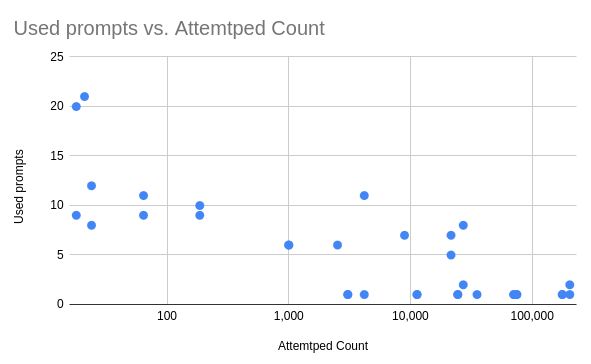
\includegraphics[width=\textwidth]{used_prompts_attempted_relation.png}
	
	It shows the relation between number of people that attempted to solve a particular problem and number of prompts that we have used to make AI solve it. As can be seen from char the general rule is that tasks attempted by smaller amount of perople was more difficult to solve by AI. We assume that this relation ocurs, because AI has less variants of training data (\textit{actual solution on CodeWars, Reddit and StackOverflow threads}). And actually we can see a breakpoint around region of 1000 attempts, where we had to increase number of prompts to solve the promlem. Due to this we have used different techniques to get problem solution from AI. Interesting fact is that even \textbf{kyu difficulty} doesn't define AI performence on task as \textbf{attempted count} do (see  \href{https://docs.google.com/spreadsheets/d/1qXPyAJsOOpmtxIoGqObwG5mTaLU3IWO0SQRGbjZPhEc/edit#gid=0}{table} from 14th to 20th row)
	
	\subsection{Generating solution to problems with big amount of attempts}
		
		Generally, we have concluded that problem that has \textbf{attempt count} bigger than 4k require one or two prompts like:
		
		\begin{itemize}
			\itemsep0em
			\item Solve this problem using python: \textbf{[provided problem statement]} and use function prototype \textbf{[function prototype]}
		   \item Your code should satisfy these test cases \textbf{[failed test cases]}
		   \item Please optimize your solution
		\end{itemize}
		
		Although there are several exceptions from this rule. Even if problem of 2 or 3d kuy has 4k attempts to solve AI (we tested this only on ChatGPT-3.5 and 4, ChatGPT has slightly lower threshold) can't solve this problem due to complexity of those problems statements and many definitions that AI fail to understand properly. Second, is that even if problems of 7, 8 kyu has small attempted count AI can solve it(see   \href{https://docs.google.com/spreadsheets/d/1qXPyAJsOOpmtxIoGqObwG5mTaLU3IWO0SQRGbjZPhEc/edit#gid=0}{table} from 14th to 20th row). 
		
		Also what we have seed is that AI sometimes can stuck on simple problem but after creating a new chat it manage to solve it after two prompts like listed above (see \href{https://docs.google.com/spreadsheets/d/1qXPyAJsOOpmtxIoGqObwG5mTaLU3IWO0SQRGbjZPhEc/edit#gid=0}{table} second row)
	
	\subsection{Generating solution to problems with small amount of attempts}
		\qquad In our tests we have seen that if problem has less than 500 \textit{sulution attempts} AI could not solve it using three types of promps listed above. AI searches for solution in the right directioin but always miss some details. So, in this case we must look for this mistakes by ourselves. For example let's take a look what we used to direct AIs to help them solve that kind of problems:
		
		\begin{itemize}
			\item\href{https://www.codewars.com/kata/57e32bb7ec7d241045000661}{Diophantine Equation Solver} is 6 kyu problem but has only \textit{64} solution attempts, so both Claude and ChatGPT-3.5 couldn't solve it just from problem statement. AIs generated right basic structure of solution, but we corrected it with proper for-loop boundaries and reminded it that he must select solutions with maximum possible $z$. After that it forgot to count all solution, so we had to remind of adding a counter too. We used the following prompts: \textit{"In fact using number theory we can prove that limit for y is math.floor(math.sqrt((z*z*z)/3))"}, \textit{"But now you must introduce a counter for all solutions"} - there were more of them but that the main ones
			\item\href{https://www.codewars.com/kata/5901aee0af945e3a35000068/train/python}{3 Matrices: Rearrange the matrix} with a difficulty of 5 kyu and 24 total solutions was solved. At first models both provided a wrong code which couldn't have been fixed. But after creating a new chat and providing libraries that should have been used, GPT-3.5 solved it at \textit{"first"} try, but Gemini couldn't solve it even that way. 
			
		\end{itemize}
		
		
		General conclusion from these examples is that AIs nowadays incapable of deep reasoning where there are no lots of similar examples. They always miss one part of solution when you ask them to fix other
	
	\subsection{Unsolved problems}
		\qquad As was mentioned before LLMs showed a poor performance on solving unpopular problems. If LLM has a little examples of similar tasks on the internet, troubles arose: at first models couldn't find an appropriate approach for the problem which led to erroneous code or incorrect solution. After few consecutive prompts providing models with failed test cases, LLMs tweaked code a little bit, but it didn't make a difference. Then we tried providing models with direct hints on approach, based on correct solutions, they rewrote code and minor part of tests passed, but they still have not been able to improve their code to work completely right. In this time there is no gain in further AI usage as we enter an cycle of same errors. We couldn't manage to solve all planned problems. You can see unsolved tasks in the \href{https://docs.google.com/spreadsheets/d/1qXPyAJsOOpmtxIoGqObwG5mTaLU3IWO0SQRGbjZPhEc/edit#gid=0}{table} (filled with grey color) 
	
	\section{Recommendations for AI code generation}
		\qquad Using collected data we created the following guidelines (algorithm) for AI code generation:
		
		\begin{enumerate}
			\item Determine if your problem is popular or totally specific
			\item If it is widespread you can just put problem statement into prompt and most likely you will get the right solution
			\item If you decided that your problem is not narrowly focuced you should:
			\begin{enumerate}
				\item Think of straighforward solution and then feed problem statement to AI
				\item Check if AI solution is going in the right direction and detemine main AI mistakes.
				\item Remind AI of those mistakes one-by-one in promts 
				\item Return to step (b) until AI returns a right solution
			\end{enumerate}
		\end{enumerate}
		
		Also don't try to feed whole problem if it has a lot of abstract definitions, classes and function that are narrowly focused to your task. Try to split problem into smaller chunks preferably to functions and solve them consequently.
		
	\section{Conclusions}
		\qquad As we have seen nowadays AI is capable of efficient problem cracking if there were lost of solutions of similar problems in the internet or they are easy enough. We cannot feed a problem with vast definitions and examples and hope that AI could understand it. Code generation can only be used to lessen the routine work of writing another one function or searching for directions in solving hard probmes as was discussed in section 2.2
	
	
\end{document}